\chapter{PBR}
PBR o \textit{physically based rendering} es el t\'ermino que se utiliza para nombrar al grupo de t\'ecnicas basados en un
modelo f\'isico. La intenci\'on de los sistemas de renderizado PBR en entornos interactivos es conseguir aproximaciones plausibles
y poco costosas de la dispersi\'on de la luz al golpear sobre una superficie. Las principales ventajas de este tipo de algoritmos
son la consistencia bajo diferentes condiciones de luz y su manejo intuitivo por parte de los artistas.\\

Las caracter\'isticas esenciales de un motor PBR, adem\'as de estar basado en la teor\'ia de microfacetas, son cumplir con el principio
de conservaci\'on de la energ\'ia y el principio de Helmholtz. Estos dos principios no siempre se cumplen en los sistemas de
de renderizado realista en entornos interactivos, que pueden presentar optimizaciones que sacrifiquen aspectos f\'isicos del modelo
en favor de tiempos de respuestas menores, siempre y cuando no resulten en artefactos apreciables.\\
% Los motores PBR cumplen con la ley de la conservaci\'on de la energ\'ia y utilizan BRDFs basados en la teor\'ia de
% microfacetas y el principio de reciprocidad de Helmholtz

Aunque este trabajo se centra en el tratamiento de materiales basados en aspectos f\'isicos, adicionalmente, otros elementos
de la escena, como la c\'amara o las luces, pueden estar basados en modelos f\'isicos para ofrecer un mayor grado de realismo.

\section{Unidades radiom\'etricas}
    % \todo[inline]{
    %     When we talk about light arriving (or leaving) a surface from a certain direction, it’s
    %     more appropriate to speak in terms of the quantity of light arriving at or passing through a
    %     certain area of space. The reason for this is that light is measured in terms of flow
    %     through an area. That is, light is measured as energy per-unit surface area (i.e.
    %     Watts/meter2). This means it doesn’t really make sense to talk about the amount light
    %     arriving from a single incoming direction – it’s more appropriate to talk about light
    %     coming from a small region of directions.
    % }
    % \todo[inline]{
    %     Since BRDFs measure how light reflects off a surface when viewed under various
    %     viewing positions, we must have a good understanding of how much light arrives at a
    %     surface element (or leaves a surface element) from a particular direction.
    % }
    Los modelos de BRDF analizados en este trabajo son basados en f\'isica y utilizan las unidades radiom\'etricas para
    medir la luz incidente o reflectada por una superficie. En estos modelos, la luz se mide como energ\'ia por unidad de
    \'area.
    % para describir la luz incidente sobre las superficies.

    \subsection*{\'Angulo s\'olido}
    El \'angulo s\'olido ($w$) es la unidad de medida del \'area de una proyecci\'on sobre una esfera de radio 1  es el
    equivalente tridimensional a la medida en radianes de un arco sobre un c\'irculo. Su unidad es el est\'ereorradi\'an
    ($sr$), que representa el \'area de un \'angulo s\'olido sobre la esfera de radio unitario $\Omega$ que contiene $4\pi$ radianes.

    \begin{figure}[H]
        \centering
          \frame{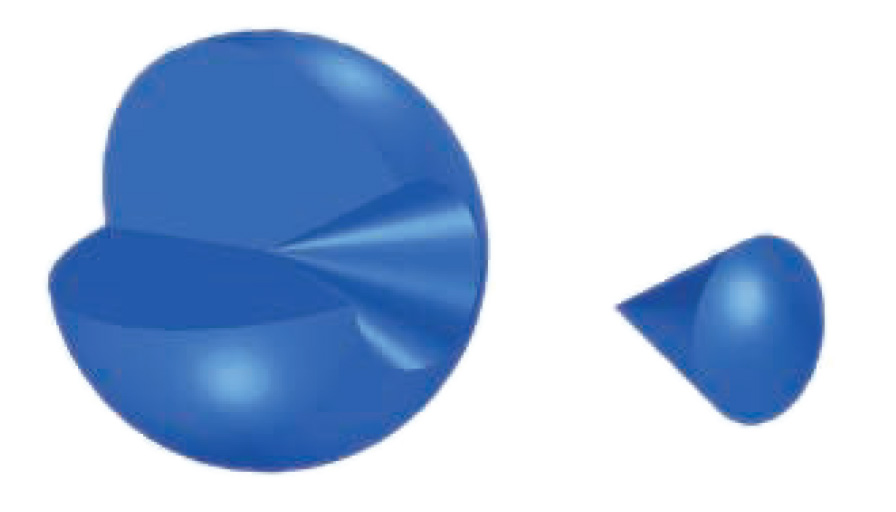
\includegraphics[scale=0.4]{steradian}}
        \caption{La superficie de la base del cono extra\'ido de la esfera representa 1$sr$.}
        \vspace{0.5cm}
    \end{figure}

    \subsection*{\'Angulo s\'olido diferencial}
    Es la unidad que se utiliza como \'area de medida en el BRDF para representar la cantidad de luz que incide en una superficie.
    Un \'angulo s\'olido diferencial ($dw$) es el \'area contenida entre incrementos muy peque\~nos en coordernadas esf\'ericas sobre
    los \'angulos $\theta$ y $\phi$ de la esfera $\Omega$.

    \begin{figure}[H]
        \vspace{0.5cm}
        \centering
          \frame{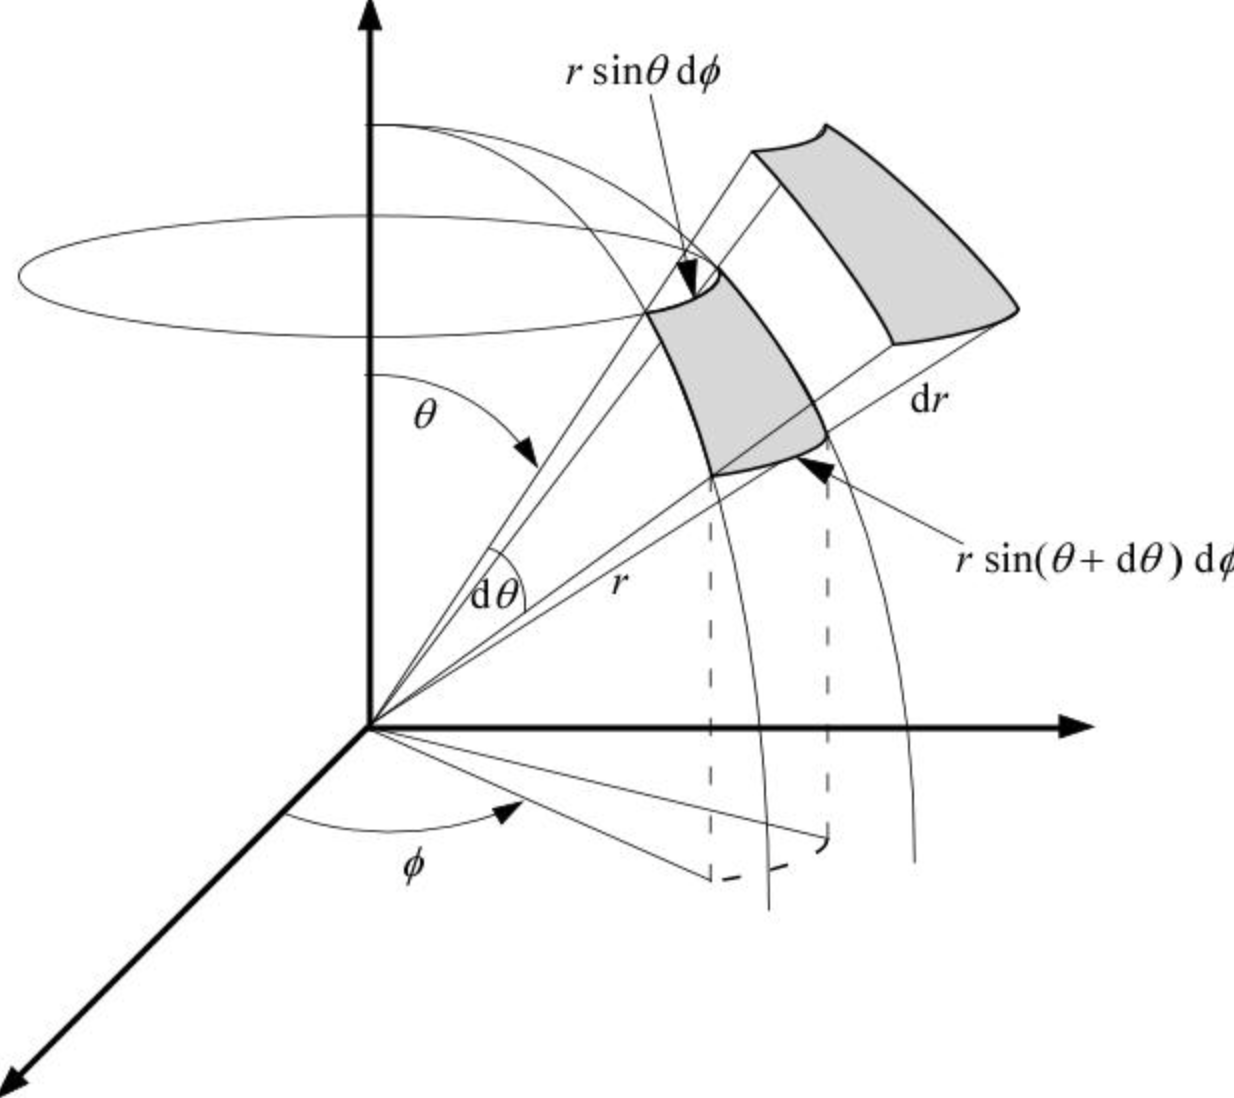
\includegraphics[scale=0.2]{differentialsolidangle}}
        \caption{Esquema explicativo de un \'angulo s\'olido diferencial.}
        \vspace{0.5cm}
    \end{figure}

    % \todo[inline]{
    %     Since both the width and the height of the rectangular patch are measured in radians, the
    %     area quantity has units of radians squared (or steradians). Steradians sounds like a fancy
    %     word, but really it’s not too bad. If ever you find the term confusing, just think of it as
    %     “solid angle units” or “radians squared”. The abbreviation for steradians is sr.
    % }

    \subsection*{Flujo radiante}
        El flujo radiante ($\Phi$) es la unidad que mide la  cantidad de energia de energ\'ia transportada
        por las ondas de luz por unidad de tiempo. En los motores de renderizado utilizan esta unidad para expresar la cantidad
        total de energia emitida por una fuente de luz y se mide en vatios ($W$).
        % \begin{equation}
        %     \Phi_e = \dfrac{d{Q_e}}{dt}
        % \end{equation}

    \subsection*{Irradiancia}
        La irradiancia ($E$) es la cantidad de energ\'ia (flujo radiante) de tiempo por unidad de superficie y
        se mide en vatios por metro cuadrado ($W/m^2$). En los motores de render se utiliza
        para medir la cantidad de luz que incide sobre un punto desde todas las direcciones.

        \begin{equation}
            E = \dfrac{d\Phi}{dA}
        \end{equation}

    \subsection*{Intensidad radiante}
        Representa el flujo radiante emitido por una fuente de luz en una direcci\'on determinada y se mide expresa
        como vatios por estereorradi\'an ($W/sr$).

        \begin{equation}
            I = \dfrac{d\Phi}{d\omega}
        \end{equation}

    \subsection*{Radiancia}
        La radiancia ($L$) se puede considerar como la combinaci\'on de los conceptos de irradiancia e intensidad radiante y
        define la direcci\'on y la intensidad radiante recibida por una superficie. La ecuaci\'on de render, igual que la c\'amaras,
        sensores o nuestros ojos miden la radiancia que llega desde las superficies del entorno al punto de vista. Su unidad son los
        vatios por metro cuadrado por estereorradi\'an (${W}/{m^2sr}$)
        \begin{equation}
            L = \dfrac{d^2\Phi}{dA_{proj}d\omega}
        \end{equation}

\section{Ecuaci\'on de render}
Presentada por primera vez en el trabajo de Kajiya \autocite{kajiya}, el prop\'osito de la ecuacion de render es conocer el valor de
radiancia que llega a la camara en una direcci\'on por cada pixel de la camara. Para ello se utiliza la ecuacion de reflectancia,
que depende de la luz que llega al punto, el coseno del angulo con el que incide la luz y el BRDF, que modela el comportamiento
de la luz al rebotar sobre la superficie.\\

\begin{eqfloat}[!htb]
    \begin{equation}
        L_o(p, w_o) = L_e(x, w_o) + \int_\Omega{f_r(p, w_i, w_o) L_i(p, w_i) n\cdot{w_i}dw_i}
    \end{equation}
  \caption{Ecuaci\'on de render}
\end{eqfloat}
\singlespacing

Siendo $L_o(p, w_o)$ la luz reflectada por la superficie, $L_e(x, w_o)$ la luz emitida por la superficie, que est\'a fuera
de la integral porque es independiente de la luz reflejada o refractada por la superficie. $\int_{\Omega}[...]dw$ que representa
que la operaci\'on se repite para cada \'angulo s\'olido dentro de la semiesfera $f_r(p, w_i, w_o)$, el BRDF, $L_i(p, w_i)$, la luz
que llega al punto de la superficie que estamos evaluando y $n\cdot{w_i}$ el factor de atenuaci\'on de la luz con respecto a la normal.

An important property of the rendering equation is that it is linear with respect to
the emitted lighting. If we make the lights twice as strong, the result of the shading will
be two times brighter. The response of the material for each light is also independent
from other sources. That is, one light’s presence does not affect the interaction of
another light with the material.\\

In real-time rendering, it is common to use just a local lighting model. Only the
surface data at visible points are needed to compute the lighting—and that is exactly
what GPUs can most efficiently provide.\\

\section{BRDF}

El BRDF, o función de ditribuci\'on bidireccional de reflectividad, es la parte de la ecuaci\'on $f_r(p, w_i, w_o)$ que describe el
comportamiento de la luz al golpear sobre la superficie y se utiliza para modelar propiedades f\'isicas de los diferentes
materiales.\\

Es una funcion estad\'istica que calcula cuanta de la luz que incide sobre un material es reflejada en direcci\'on
a la c\'amara, para ello toma como argumentos la direccion de la luz, $w_i$, y la dirección de salida,
$w_o$, la normal de la superficie, $n$, y un par\'ametro $\alpha$ que representa la rugosidad del material.

\begin{figure}[H]
    \vspace{0.5cm}
    \centering
      \frame{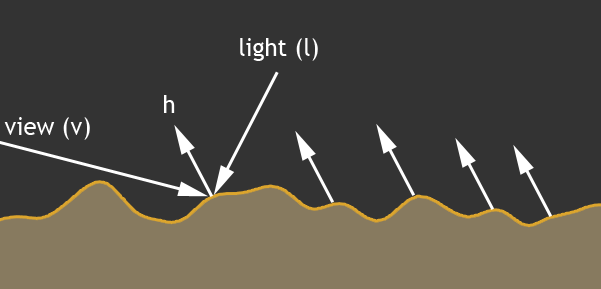
\includegraphics[scale=0.7]{microfacet-diagram}}
    \caption{Diagrama de la luz incidente y luz reflectada}
    \vspace{0.5cm}
\end{figure}

Para que un BRDF se considere como PBR, ha de utilizar el modelo de microfacetas, ademas de cumplir con la ley de conservacion
de la energia, $\forall w_i \int_{\Omega} f(p, w_i, w_o) n\cdot{w_i} dw_o \leq 1$ y el principio de reciprocidad de Helmholtz,
el BRDF debe de ser simétrico, esto es que invertir la direccion de entrada y salida del BRDF no deberia afectar al resultado
$f(x, w_i, w_o) = f(x, w_o, w_i)$ sin embargo, los motores en tiempo real, frecuentemente incumplen el principio de reciprocidad,
no siendo fisicamente plausibles, pero sin generar artefactos.\\

    \subsection{Teor\'ia de microfacetas}

    \bgroup

        Aunque a escala macrosc\'opica podamos considerar una superficie como lisa, ninguna superficie es completamente lisa a nivel
        microsc\'opico. La teor\'ia de microfacetas utiliza una representaci\'on estad\'istica para modelar estas peque\~nas irregularidades.\\

        La teor\'ia de microfacetas, considera la superficie de reflexi\'on como una superficie compuesta por una matriz de
        superficies mas peque\~nas que la longitud de onda de la luz pero muy peque\~nas desde el punto de vista de la c\'amara,
        completamente reflectantes, llamadas microfacetas, y cuyas diferentes orientaciones determinan la rugosidad de la superficie.
        Si las microfacetas est\'an completamente alineadas, las reflexiones ser\'an mas definidas, asimilandose a un espejo, mientras
        que las microfacetas apuntando en diferentes direcciones, dar\'an como resultado una reflexion especular mas difusa.

        \begin{figure}[H]
            \vspace{0.5cm}
            \centering
            \frame{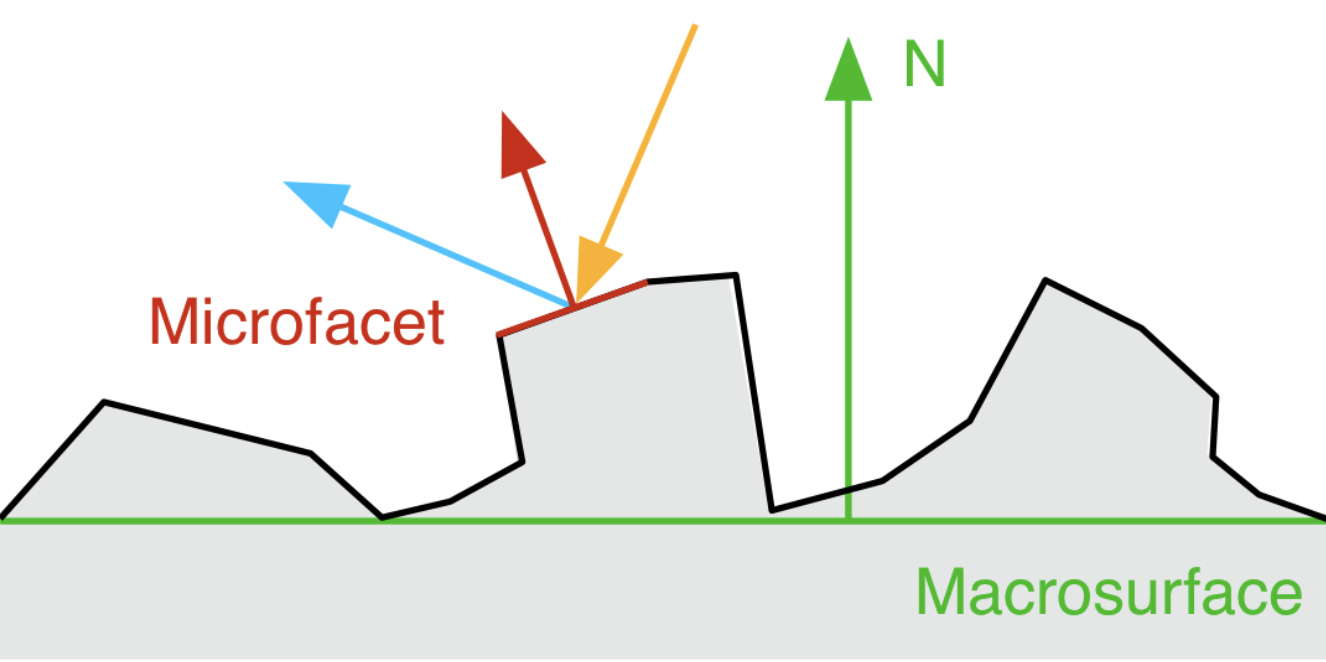
\includegraphics[scale=0.55]{macrosuperficie}}
            \caption{Superficie a escala microsc\'opica}
            \vspace{0.5cm}
        \end{figure}

    \egroup


    \subsection{Tipos de BRDFs}
    Existen diferentes tipos de BRDFs en funci\'on de las propiedades f\'isicas del material que se quiera representar. Los
    materiales met\'alicos utilizan un BRDF diferente a los diel\'ectricos, esto es as\'i porque los efectos de absorci\'on y
    dispersi\'on, son completamente diferentes en funci\'on de esta propiedad.\\

    En los materiales metalicos, la reflexi\'on especular es de color, la luz refractada es absorbida por el propio material
    y no existen efectos de dispersi\'on de la luz bajo la superficie, mientras que en los materiales diel\'ectricos, o no
    met\'alicos, el aspecto final del material esta determinado por una combinaci\'on de los fen\'omenos de absorci\'on y
    dispersi\'on de la luz.\\

    Por otra parte, podemos diferenciar entre materiales anisotr\'opicos, como el metal pulido o el pelo, cuyas propiedades
    de reflexi\'on cambian al rotar sobre la superficie alrededor de su vector normal. Aunque casi todos los materiales son, en cierta medida, anisotr\'opicos, la
    aportaci\'on de esta propiedad sobre la apariencia final suele ser tan baja que se desprecia y se utilizan modelos
    isotr\'opicos.\\

    Adem\'as, seg\'un su origen, podemos distinguir principalmente entre tres tipos de modelos: emp\'iricos, te\'oricos y
    experimentales. Los modelos emp\'iricos no est\'an basados en f\'isica, si no que son simplificaciones de menor coste que
    aproximan un determinado fen\'omeno, ejemplos de modelos emp\'iricos son los modelos de Phong \autocite{phong} o el
    de Blinn-Phong \autocite{blinnphong}. Los modelos te\'oricos, como los basados en microfacetas, se basan en observaciones sobre el comportamiento de la luz y su
    interacci\'on sobre las superficies para crear un sistema de ecuaciones que describan este comportamiento sobre un modelo
    matem\'atico. Por \'ultimo, los modelo experimentales, se basan en datos de estudios experimentales con la luz a partir de los
    que crean funciones que se ajustan a los datos obtenidos en dichos estudios, el BRDF de Schlick es un ejemplo de modelo
    experimental.
    % Los diferentes tipos de BRDFs permiten para modelar diferentes propiedades de los materiales, isotropia o anisotropia,
    % transmitancia, reflexiones internas, etc. Podemos clasificar los diferentes tipos de BRDFs entre modelos analiticos y BDRFs
    % de datos adquiridos. Los modelos analiticos son funciones matemáticas que modelan diferentes efectos de la luz en funcion de
    % sus datos de entrada, mientras que los BRDFs de datos adquiridos, capturan el BRDF de un material con un gonioreflectometro,
    % y permiten una representacion muy precisa del material escaneado.

    % Comunmente, en la industria se utilizan modelos anal\'iticos, debido a su flexibilidad y rendimiento y el mas utilizado a
    % d\'ia de hoy en la industria, aunque con algunas variaciones en sus t\'erminos, sigue siendo el modelo de Cook-Torrance\autocite{cooktorrance}.
    % \todo[inline]{
    %     Metal. The appearance of the metal mainly depends on the direct reflection of light at the interface of the two media (ie, specular reflection). The metallic specular reflection color is a three-channel color, and R, G, and B are different. The light refracted into the metal is almost immediately absorbed by free electrons, and there is no scattering of light refracted into the metal.
    %     Non-Metal. Non-metal is a dielectric, and its overall appearance is mainly determined by its combination of absorption and scattering characteristics. Similarly, the interaction between non-metal and light is divided into reflection and refraction. According to the scattering and absorption characteristics of the medium type, refraction is divided into multiple categories:
    % }
    % \todo[inline]{
    %     The term isotropic is used to describe BRDFs that represent reflectance properties that
    %     are invariant with respect to rotation of the surface around the surface normal vector.
    %     Consider a small relatively smooth surface element and fix the light and viewer positions.
    %     Anisotropy, on the other hand, refers to BRDFs that describe reflectance properties that
    %     do exhibit change with respect to rotation of the surface around the surface normal
    %     vector. Some examples of materials that have anisotropic BRDFs are brushed metal,
    %     satin, and hair.
    % }

    \begin{figure}[H]
        \centering
        \frame{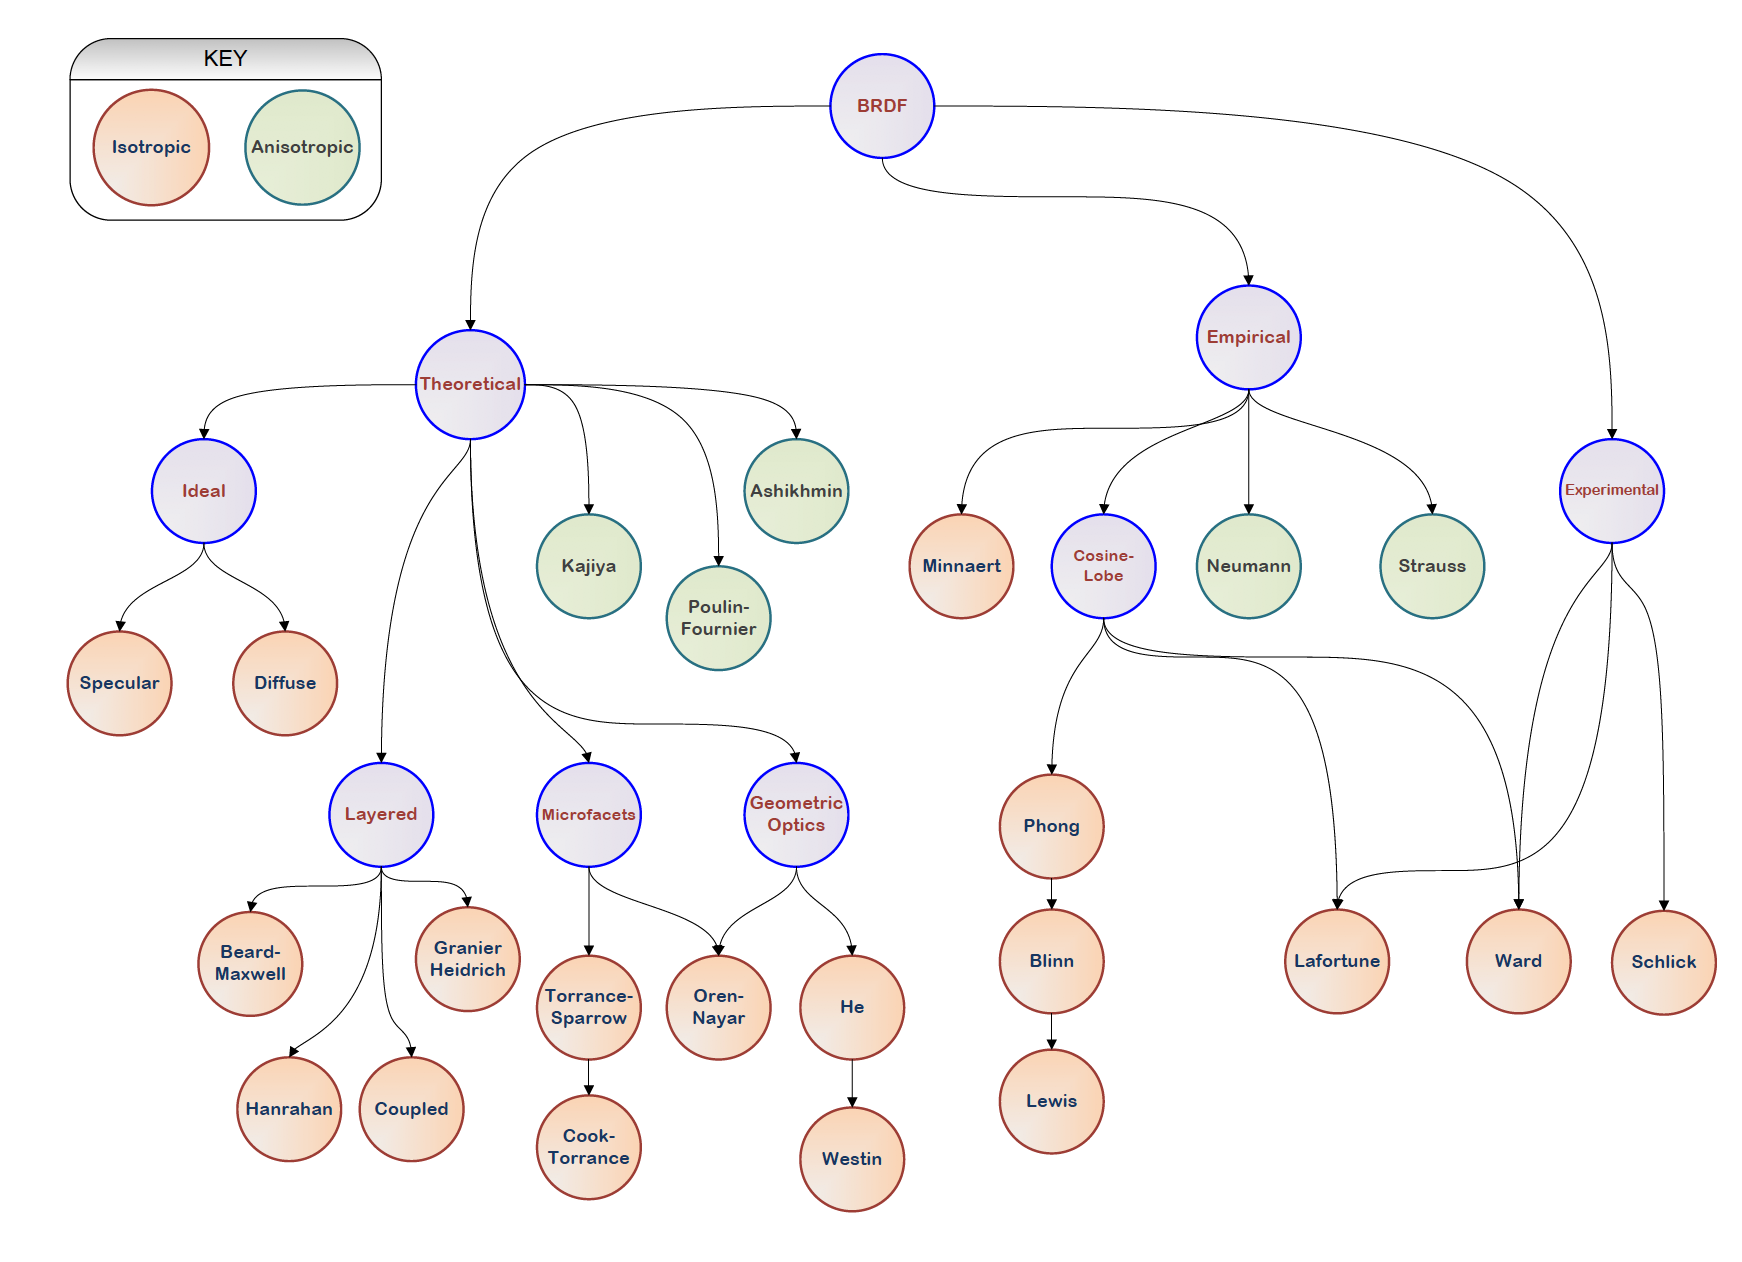
\includegraphics[scale=0.45]{schema_brdfs}}
        \caption{Esquema de diferentes modelos de BRDF seg\'un su origen}
        \vspace{0.5cm}
    \end{figure}

    \section{BRDF Cook-Torrance}
    Es un modelo anal\'itico permite representar con gran realismo materiales electricos y dielectricos con diferentes
    grados de rugosidad y, en general, funciona bien para modelar cambios en el color que dependen del punto de vista.\\
    Este modelo permite estudiar por separado las dos componentes de la luz, especular y difuso:
    
    \begin{eqfloat}[!htb]
        \begin{equation}
            f_r = k_{d}f_{lambert} + k_sf_{cook-torrance}
        \end{equation}
        \caption{BRDF como suma de la componente difusa y especular}
    \end{eqfloat}
    
    siendo $k_d$ y $k_s$, parametros de peso que cumplen $k_d + k_s = 1$
    \singlespacing

    \begin{figure}[H]
        \vspace{0.5cm}
        \centering
        \frame{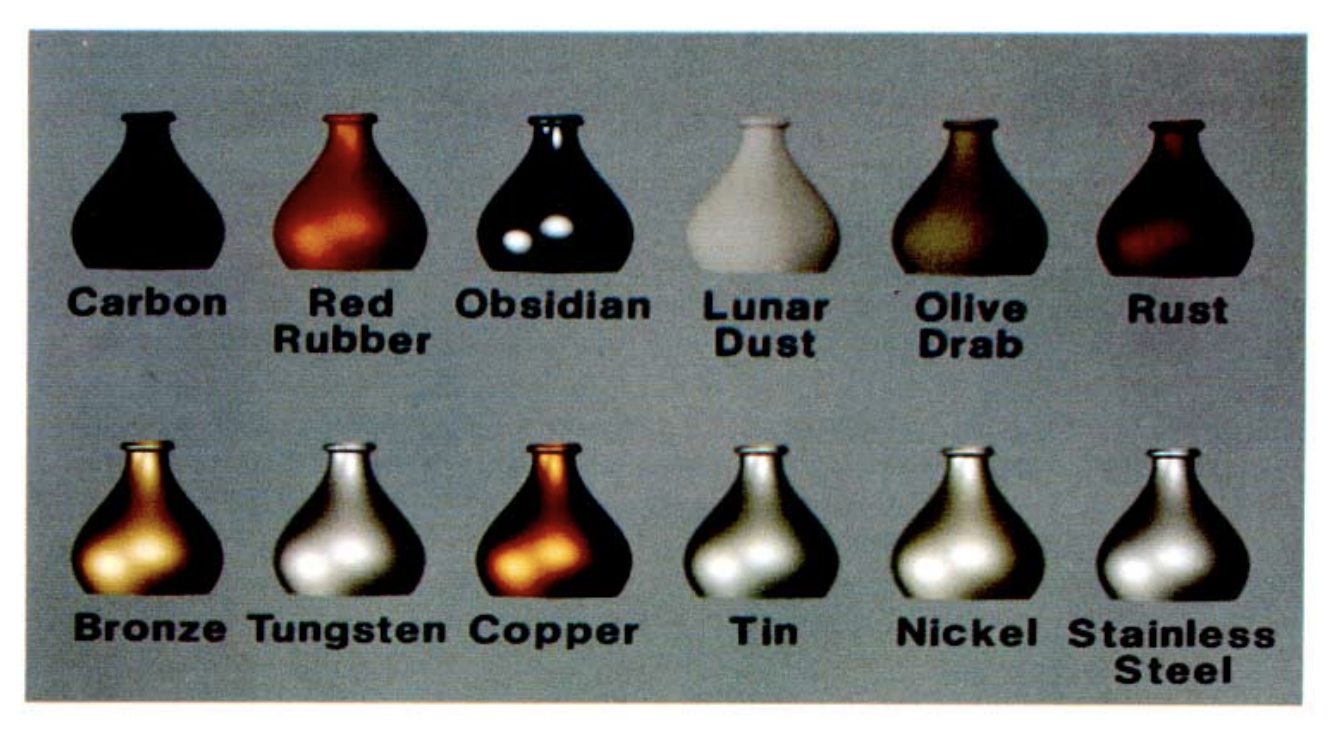
\includegraphics[scale=0.5]{cooktorrance}}
        \caption{Diferentes tipos de materiales representados por el modelo de Cook-Torrance \autocite{cooktorrance}}
        \vspace{0.5cm}
    \end{figure}
    
    T\'ipicamente la componente difusa, utiliza el modelo de Lambert, que asume una distribuci\'on completamente uniforme a lo
    largo de la superficie:\\
    
    \begin{equation}
    f_{Lambert} = \frac{diffuse}{\pi}
    \end{equation}
    \singlespacing
    
    La componente especular es una funci\'on compuesta de otras tres funciones y un factor de normalizaci\'on en el
    denominador.\\
    
    \begin{equation}
        f(l, v) = \frac{F(w_i, h) G(w_i, h, w_o) D(h)} {4(n\cdot{w_i}) (n \cdot{w_o})}
    \end{equation}
    \singlespacing

    \begin{figure}[H]
        \centering
        \frame{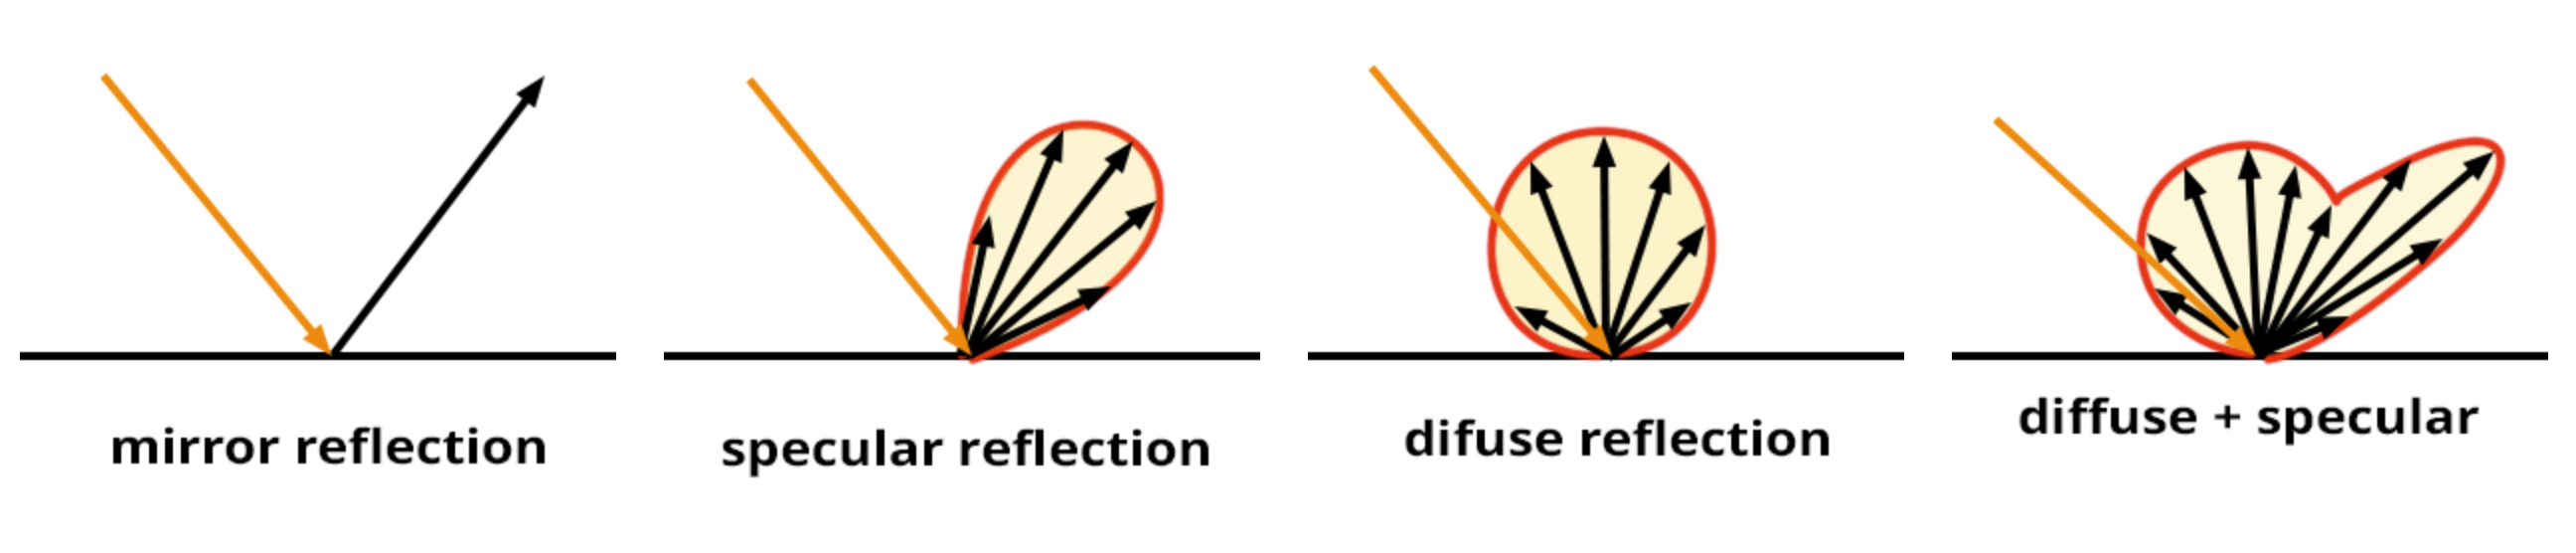
\includegraphics[scale=0.32]{diffusespecular}}
        \caption{Tipos de reflexi\'on}
        \vspace{0.5cm}
    \end{figure}
    
        \subsection{Componente especular}
            El BRDF de Cook-Torrance est\'a compuesto por otras tres funciones y un factor de normalizaci\'on en el denominador.
            Las funciones D, F y G, se corresponden con la funci\'on de distribuci\'on de las normales, la ecuaci\'on de Fresnel,
            y la funci\'on de geometr\'ia.\\
    
            $D(l, v, h)$  es la funci\'on de distribuci\'on de las normales y se encarga de representar la rugosidad de una superficie
            y es el t\'ermino que afecta en mayor grado a la forma y taman\~no del brillo especular. T\'ipicamente el par\'ametro
            \textit{roughness} se utiliza para representar la cantidad de microfacetas alineadas con la normal h, cuanta mayor sea la
            la cantidad de de microfacetas alineadas, m\'as lisa parecer\'a la superficie.
    
            \singlespacing
            \begin{equation}
            D(h) = \frac{\alpha^2}{\pi((n\cdot{h})^2(\alpha^2 - 1) + 1)^2}
            \end{equation}
            \singlespacing
            
    
            \begin{figure}[H]
                \vspace{0.5cm}
                \centering
                \frame{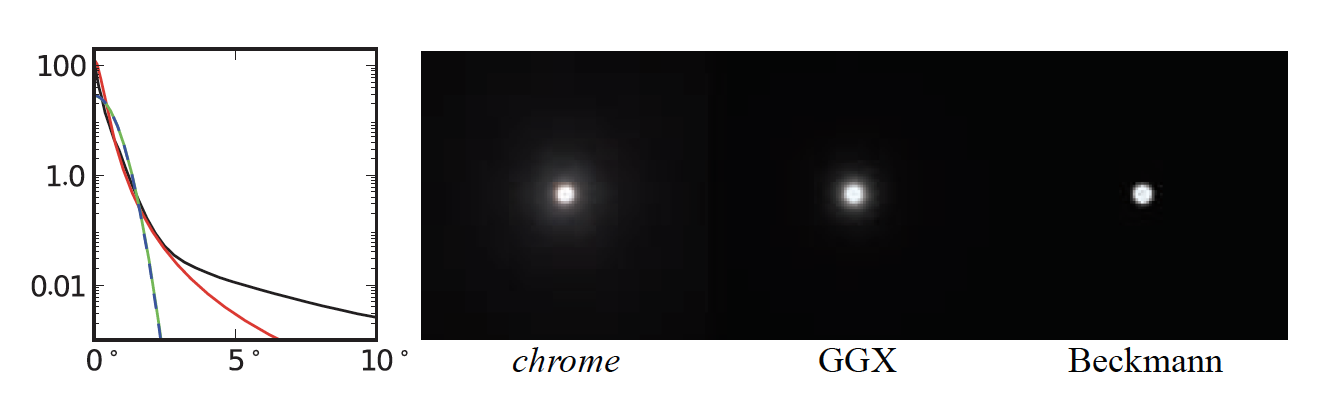
\includegraphics[scale=0.65]{ndf}}
                \caption{Representaci\'on gr\'afica de la funci\'on de geometr\'ia}
            \end{figure}
    
            $G(w_o)$ es la funci\'on de geometr\'ia. Esta funci\'on tiene en cuenta las oclusiones debidas a la propia superficie.
            Mientras que el t\'ermino de distribucion de las normales, $D(h)$, define la concentraci\'on de microfacetas con una normal h,
            no define si esas microfacetas son visible o no. El t\'ermino de geometr\'ia tiene en cuenta las dos cosas, la sombra
            y el enmascaramiento. La sombra representa que una microfaceta no es visible desde la direcci\'on de la luz, mientras que el
            enmascaramiento significa que una microfaceta no es visible desde la direcci\'on de vista y, por tanto, no contribuyen
            a la reflexi\'on.
    
            $$
            G(w_i, w_o) = G(w_i)G(w_o)
            $$
            \singlespacing
            $$
            G(w_o) = \frac{n\cdot{w_o}}{(n\cdot) (1 - k) + k}
            $$
            \singlespacing
            $$
            G(w_i) = \frac{n\cdot{w_i}}{(n\cdot) (1 - k) + k}
            $$
            \singlespacing
    
            \begin{equation}
            k = \frac{(roughness + 1)^2}{8}
            \end{equation}
    
            \begin{figure}[H]
                \vspace{0.5cm}
                \centering
                \frame{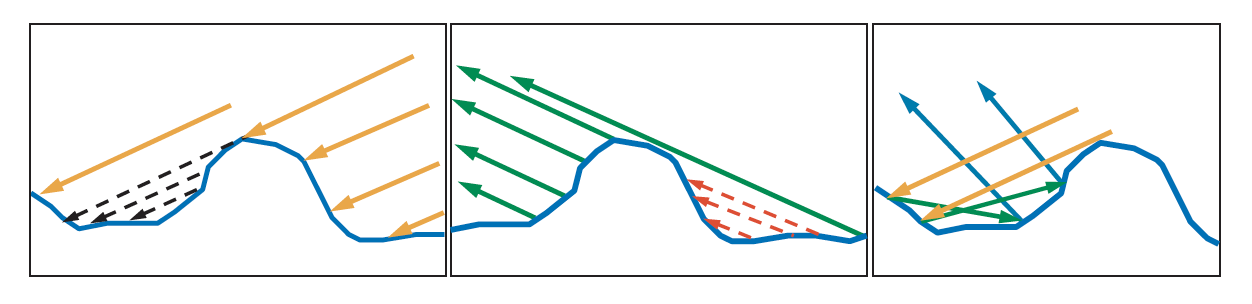
\includegraphics[scale=0.65]{microgeometria}}
                \caption{Representaci\'on gr\'afica de la sombra y el enmascaramiento en la funci\'on de geometr\'ia}
            \end{figure}
    
            $F(l, v, h)$ es la funci\'on de Fresnel. Representa la radiancia reflejada por un material seg\'un el \'angulo de incidencia
            de la luz. Para la mayor\'ia de los materiales no met\'alicos, las reflexiones son m\'as intensas bajo cuando el \'angulo
            de incidencia es muy agudo. En la mayor\'ia de los algoritmos de sombreado, el fresnel se utiliza a nivel de la macrosuperficie,
            sin embargo, al aplicar el fresnel sobre la normal de la microfacetas, se consigue un mayor grado de realismo para los valores
            altos de \textit{roughness}.
    
            $$
            F_{Schlick}(F_o, w_i, h) = F_o + (1 - F_o) (1 - (l\cdot{h}))^5
            $$
    
            \begin{figure}[H]
                \vspace{0.5cm}
                \centering
                \frame{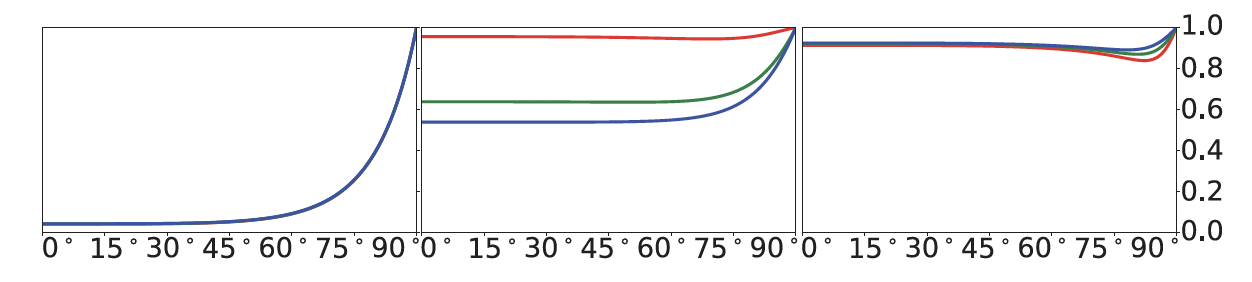
\includegraphics[scale=0.65]{fresnel}}
                \caption{Representaci\'on gr\'afica de la funci\'on de geometr\'ia}
            \end{figure}
            \singlespacing
    
            El denominador es una caracter\'istica t\'ipica de los modelos de microfacetas y es un factor de correci\'on debido al cambio
            de espacio entre el espacio local de las microfacetas y el espacio local de la macrosuperficie. Para modelos que no
            incluyen este factor, se puede aplicar un factor de sombreado directamente multiplicando el t\'ermino de geometr\'ia por
    
            \begin{equation}
            \frac{1}{4(n\cdot{l}) (n\cdot{v})}
            \end{equation}
            \singlespacing
    
            % La funci\on de distribuci\'on de las normales, aproxima la cantidad de microfacetas aproxima la alineadas con el
            % vector h, el medio entre el rayo de luz y el punto del vista. El par\'ametro que modela la rugosidad de una superficie
            % afecta en gran medida al resultado. Este es el factor m\'as caracter\'istico del modelo de microfacetas.
            % La funci\'on de geometr\'ia describe la cantidad de rayos ocluidos por las propias microfacetas.\\
    
            % Finalmente, la ecuaci\'on de fresnel describe el ratio de reflexi\'on de una superficie bajo diferentes \'angulos de
            % incidencia.\\
    
    \section{Disney Principled BRDF}
    Los modelos de BRDF para materiales tratan de ofrecer gran versatilidad para tratar de representar la mayor cantidad de
    materiales posibles, por lo que los modelos basados en f\'isica resultan en una defici\'on del material compleja,
    con gran cantidad de par\'ametros que resultan poco intuitivos para los artistas. En 2012, Disney presenta su modelo
    conocido como \textit{Principled} \autocite{disney12}, que, a pesar de ser basado en f\'isica, sigue una serie de directivas
    como tener la menor cantidad de par\'ametros posibles, ofrecer nombres y rangos de par\'ametros amigables para los artistas u ofrecer
    combinaciones robustas y plausibles para todas sus posibles combinaciones. Desde entonces, los materiales basados en f\'isica
    han ganado popularidad y se han introducido progresivamente en la industria de las pel\'iculas y videojuegos, convirtiendo
    al modelo de Disney en el est\'andar de facto en la actualidad.\\

    \begin{figure}[H]
        \vspace{0.5cm}
        \centering
        \frame{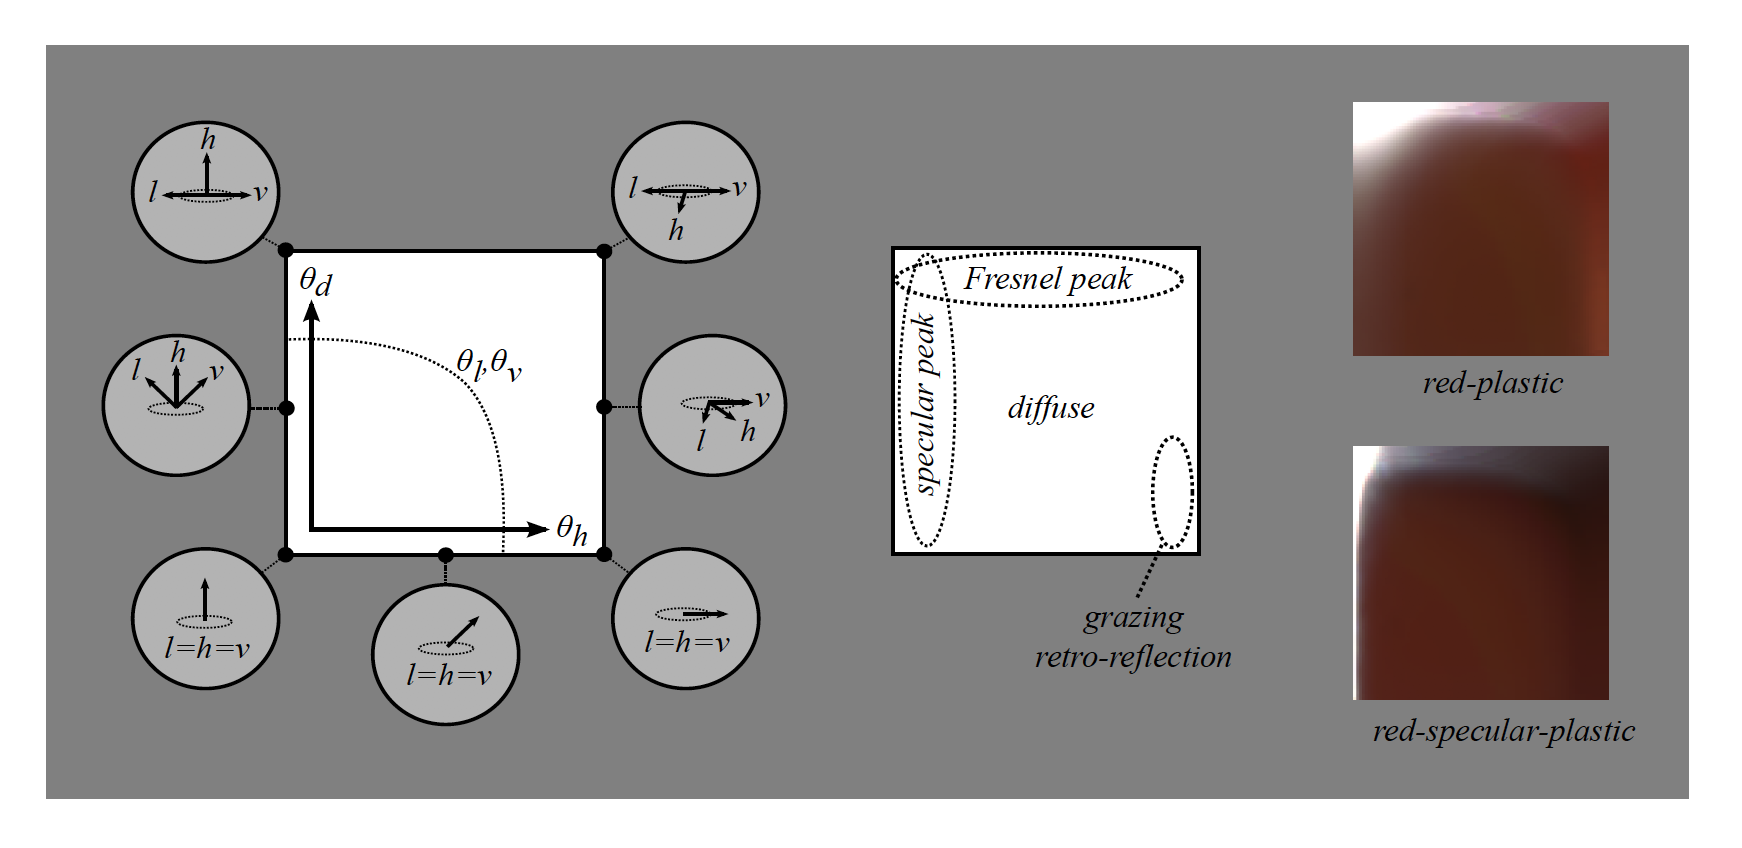
\includegraphics[scale=0.47]{slicespace}}
        \caption{Muestras de materiales MERL, junto a un esquema explicativo de las im\'agenes muestreadas}
        \vspace{0.5cm}
    \end{figure}

    El modelo te\'orico de Disney est\'a basado en las observaciones sobre la tabla MERL \autocite{merl}, que provee una lista
    de 100 materiales muestreados y representados en una gr\'afica cartesiana, cuyo eje $x$ representa pasos discretos de rotaci\'on
    alrededor de la tangente del material y en el $y$, la rotaci\'on alrededor de la normal de la superficie. 

    \begin{figure}[H]
        \vspace{0.5cm}
        \centering
        \frame{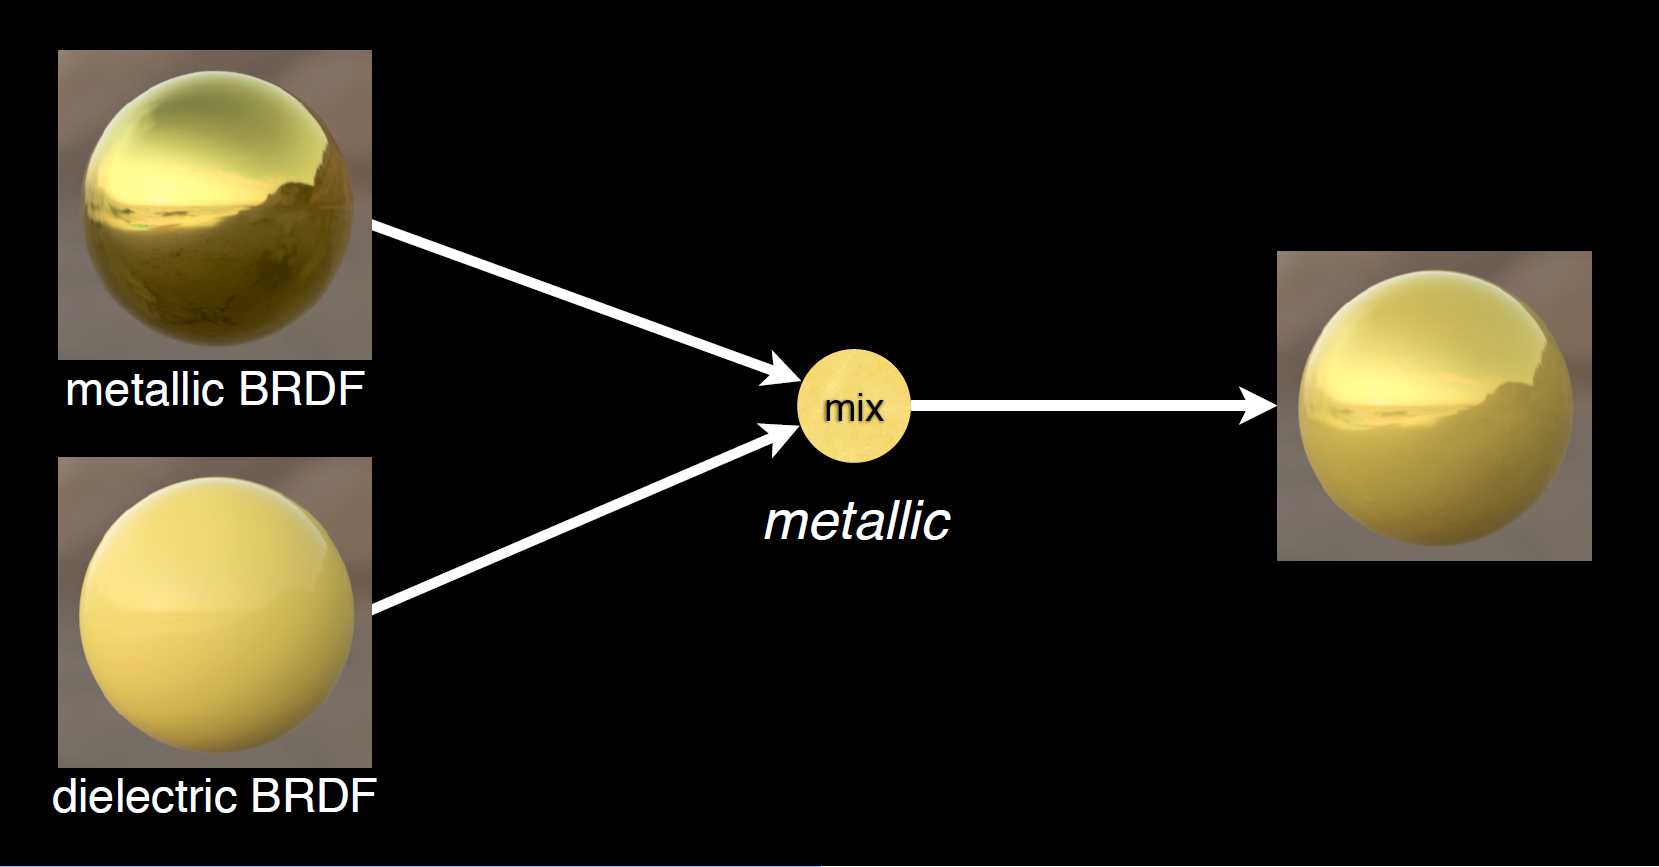
\includegraphics[scale=0.3]{disney12model}}
        \caption{Modelo para met\'alicos y diel\'ectricos de Disney}
    \end{figure}

    En base a estas observaciones, el modelo \textit{Principled} de Disney, ajusta los t\'erminos del BRDF de Cook-Torrance \autocite{cooktorrance}
    primando la expresividad art\'istica sobre lo f\'isicamente plausible. El modelo aporta dos nuevos l\'obulos que, a diferencia del l\'obulo
    primario pueden variar mucho en forma y tama\~no, adem\'as los tanto los materiales isotro\'opicos como anisotr\'opicos
    se representan con el mismo modelo, que utiliza una interpolaci\'on entre los dos BRDFs, por lo que resulta muy atractivo para los artistas,
    pudiendo representar una enorme variedad de materiales con muy pocos par\'ametros.\\

    La lista de par\'ametros final se compone de: \textit{baseColor}, \textit{subsurface}, \textit{metal}, \textit{specular}, \textit{specularTint},
    \textit{roughness}, \textit{sheen}, \textit{sheenTint}, \textit{clearCoat}, \textit{clearcoatGloss}
    
    % El BRDF de Disney fue presentado por Brent Burley en 2012 y es el utilizado por Disney en sus peliculas de animacion. Es,
    % junto al modelo de Cook-Torrance, el mas utilizado en los motores de tiempo real, sin embargo, el modelo de Burley, es mas
    % amigable para los artistas, a costa de no ser completamente basado en fisica. Los parametros tienen nombres y valores que
    % definen que el aspecto de los materiales son mas intuitivos. Los lobulos adicionales, a diferencia del modelo de Cook-Torrance,
    % pueden variar mucho en forma y tamanho, por lo que es un modelo muy flexible, que permite representar con gran realismo una
    % amplia variedad de materiales.\\
    
    % Es conocido como \textit{principled} por cumplir una serie de m\'aximas, que se respetan en el modelo por encima de las leyes fisicas.
    % El modelo ha de ser intuitivo y no utilizar parametros que se refieran al modelo basado en fisica, debe tener el menor
    % numero de parametros posible, deben de estar normalizados, algunos valores pueden exceder su rango para permitir mayor
    % expresividad y, finalmente, todas las combinaciones de parametros deben de ser robustas y plausibles. Para ello utiliza los
    % par\'ametros: \textit{baseColor}, \textit{subsurface}, \textit{metal}, \textit{specular}, \textit{specularTint}, \textit{roughness},
    % \textit{sheen}, \textit{sheenTint}, \textit{clearCoat}, \textit{clearcoatGloss}
    
    \begin{figure}[H]
        \vspace{0.5cm}
        \centering
          \frame{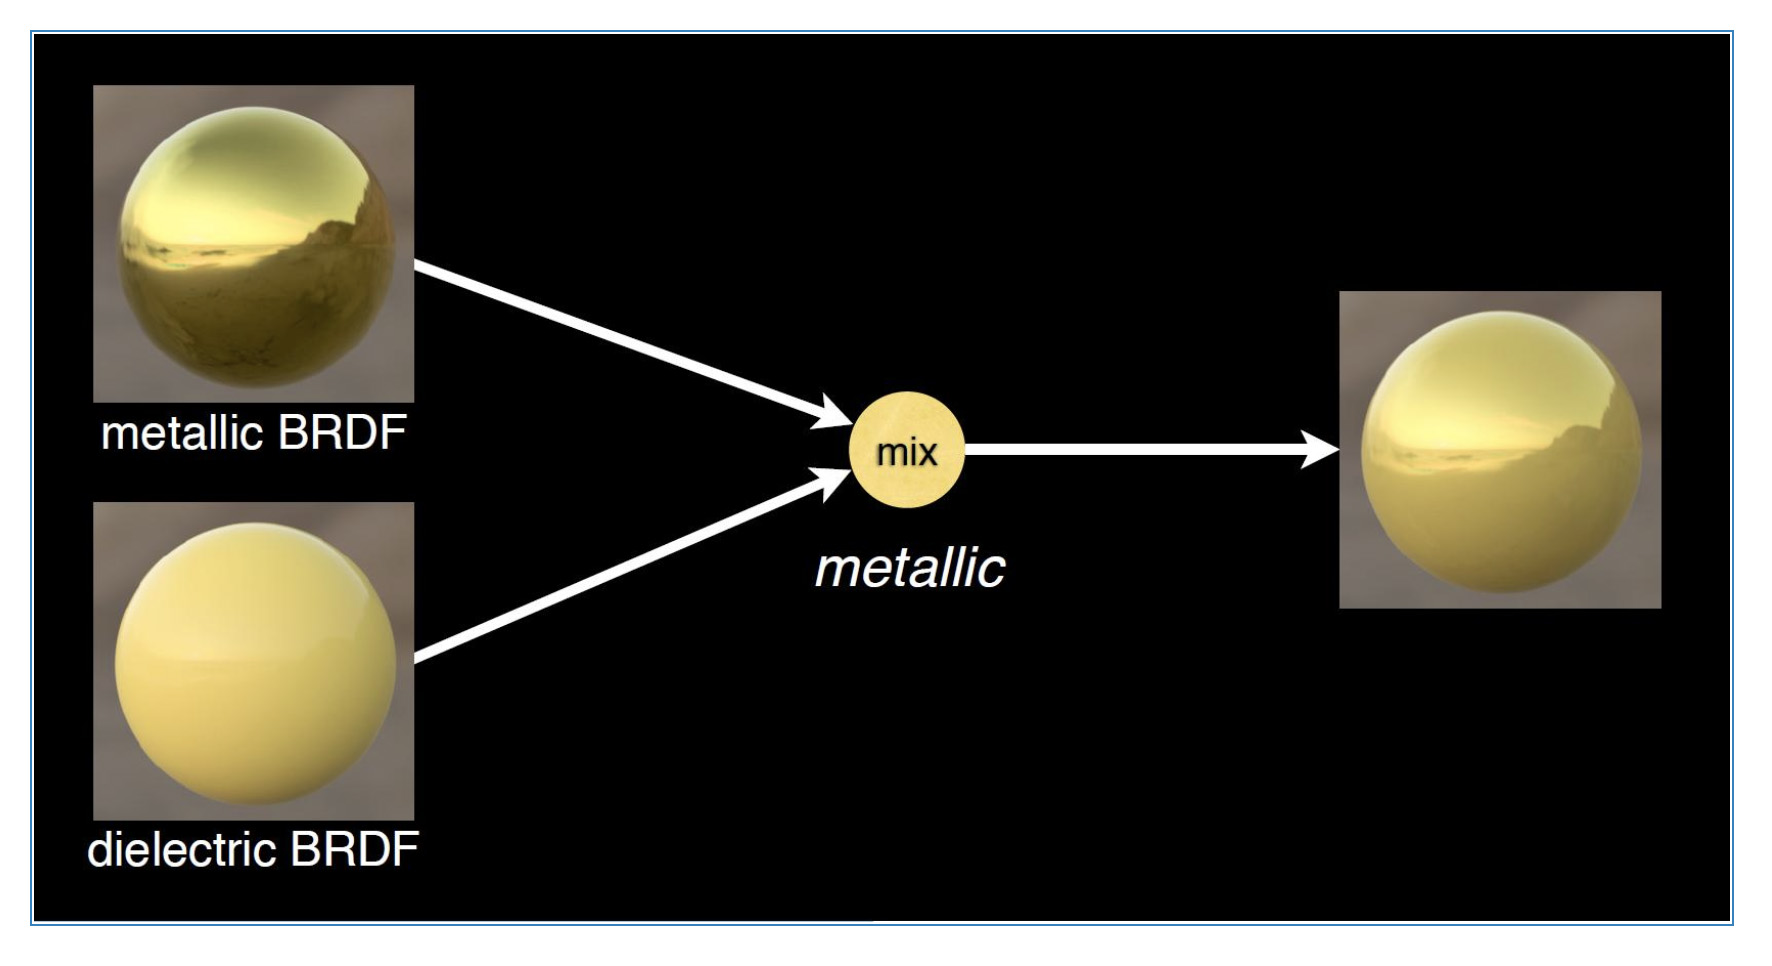
\includegraphics[scale=0.47]{disney}}
        \caption{Modelo de Disney}
    \end{figure}
    % \begin{itemize}
    % 	\item \textit{baseColor}: el color de la superficie, comunmente utiliza un mapa.
    % 	\item \textit{subsurface}: aproximacion para controlar el color de la reflexion difusa.
    % 	\item \textit{metal}: interpolaci\'on lineal entre los dos modelos. El met\'alico no tiene
    %     componente de reflexi\'on difusa y su componente de reflexi\'on especular es del mismo color que el color base. 
    %     \item \textit{specular}: cantidad de luz incidente reflejada, se utiliza para controlar de forma intuitiva el \'indice de refracci\'on de
    %     una superficie.
    % 	\item \textit{specularTint}: par\'ametro que permite a los artistas controlar el color de la reflexi\'on especular sobre el color
    % 	base.
    % 	\item \textit{roughness}: describe la rugosidad de una superficie, afectando a la reflexi\'on difusa y especular.
    % 	\item \textit{sheen}: permite mayor grado de control sobre la reflexi\'on especular, muy \'util sobre tejidos.
    % 	\item \textit{sheenTint}: color del \textit{sheen}
    % 	\item \textit{clearCoat}: un l\'obulo extra.
    % 	\item \textit{clearcoatGloss}: permite controlar la rugosidad de este l\'obulo.
    % \end{itemize}
        
        \subsection{Componente difusa}
    
        En base a las observaciones sobre los datos de MERL, el modelo difuso parece muy oscuro hacia los bordes, y aplicando
        la funci\'on de Fresnel, para intentar conseguir un modelo f\'isicamente plausible, parece oscurecer m\'as los bordes,
        acentuando el problema. Disney desarroll\'o un modelo emp\'irico, que utiliza la aproximaci\'on de Fresnel Schlick:
    
        \begin{equation}
            (1 - F(\theta_l) (1 - F(\theta_d)))
        \end{equation}
        \singlespacing
    
    
        Modific\'andolo para conseguir que la retrodispersi\'on dependa del valor de \textit{roughness} y as\'i
        adaptarse mejor a los datos obtenidos de MERL.
    
        \begin{equation}
        f_d = \frac{baseColor}{\pi}
        \left(  1 + (F_{D90} - 1)(1 - cos\theta_{wi})^5  \right)
        \left(  1 + (F_{D90} - 1)(1 - cos\theta_{wo})^5  \right)
        \end{equation}
        
        $$
        F_{D90} = 0.5 + 2roughness\cdot{cos^2\theta_d}
        $$
    
        \subsection{Componente especular}
            % \todo[inline]{Por escribir}
            \subsubsection{F, t\'ermino de Fresnel}
                Para el especular, la aproximaci\'on de Fresnel Schlick es lo suficientemente precisa y mucho menos costosa que
                que la ecuaci\'on completa de Fresnel.
    
                \begin{equation}
                (1 - F(\theta_l) (1 - F(\theta_d)))^5
                \end{equation}
    
                $F_0$ representa la reflectancia de una incidencia del mismo \'angulo que la normal. $\theta_d$ es el \'angulo
                entre el vector $h$, y el de vista $w_o$. Es acrom\'actico para los diel\'ectricos y crom\'atico para los metales.
    
            \subsubsection{G, t\'ermino de geometr\'ia}
                En el t\'ermino G, Disney utiliza dos modelos diferentes, uno para el l\'obulo primario y otro para el de clearcoat.
                Para el l\'obulo primario, utiliza el modelo de Smith GGX, remapeando el valor de \textit{roughness} para evitar
                ganar demasiada energ\'ia hacia los bordes de materiales brillantes.
    
                $$
                G(l, v, h) = G_{GGX}(l)G_{GGX}(v)
                $$
    
                $$
                G_{GGX}(v) = \frac
                {2 (n \cdot{v})}
                {(n \cdot{v}) + \sqrt{ \alpha^2 + (1 - \alpha)^2 (n \cdot{v})^2 }}
                $$
    
                \begin{equation}
                \alpha = (0.5 + roughness / 2)^2
                \end{equation}
                \singlespacing
    
                Para el l\'obulo secundario se utiliza un valor fijo de $\alpha = 0.25$.
    
            \subsubsection{D, t\'ermino de distribuci\'on de las normales}
                La distribuci\'on GGX es equivalente a la de Trowbridge-Reitz, no tiene una cola lo suficientemente larga para la
                mayor\'ia de materiales.
    
                \begin{equation}
                    D_{TR} = \frac
                    {c}
                    {(\alpha^2 cos^2 \theta_h + sin^2 \theta_h)^2}
                \end{equation}
                \singlespacing
    
                El modelo de Disney utiliza un exponente en el denominador que permite mayor control sobre el radio de la reflexi\'on
                especular, llamando a \'este t\'ermino Generalized Trowbridge-Reitz, o GTR:
    
                \begin{equation}
                    D_{GTR} = \frac
                    {c}
                    {(\alpha^2 cos^2 \theta_h + sin^2 \theta_h)^\gamma}
                \end{equation}
                \singlespacing
    
                Los dos l\'obulos, primario y secundario utilizan la distribuci\'on GTR. El l\'obulo primario,
                que representa la reflexi\'on del material base, utiliza $\gamma = 2$ y puede ser diel\'etrico o met\'alico,
                isotr\'opico o anisotr\'opico. Por otra parte, el l\'obulo secundario representa la capa de \textit{clearcoat}
                sobre el material base, utiliza $\gamma = 1$ y suele ser isotr\'opico y no met\'alico.
    
    
    
    \section{Iluminaci\'on indirecta en tiempo real}

    \todo[inline]{
        Los motores de renderizado en tiempo real deben utilizar algoritmos lo menos costosos posibles para garantizar un buen
        tiempo de respuesta. Es por ello que sus BRDFs, pueden ser m\'as sencillos que los implementados en sistemas de \textit{path-tracing},
        ofreciendo una soluci\'on de compromiso entre el rendimiento y los fen\'omenos f\'isicos representados por el modelo.\\
        
        Por otra parte, resolver la parte integral de la ecuaci\'on de render:
    
        \begin{center}$L_o(p, w_o) = \int_{\Omega} f_r(p, w_i, w_o)L_i(p, w_i)n\cdot{w_i}dw_i$\end{center}
        \singlespacing
        requiere lanzar rayos no en una direcci\'n si no desde todas las posibles direcciones sobre la semiesferea $\Omega$, por
        lo que no es posible en tiempo real, sin embargo, m\'as adelante analizaremos t\'ecnicas que p\'ermiten simular \'este
        efecto utilizando c\'alculos precomputados o aproximando la soluci\'on de forma anal\'itica.\\
    }

    \todo[inline]{
        These effects contribute
        greatly to increasing the realism in a rendered image, and provide cues that
        help the viewer to understand spatial relationships. At the same time, they are also
        complex to simulate and might require precomputations or rendering multiple passes
        that compute some intermediate information.
    }


    Para los efectos de iluminacion global, se necesita conocer la irradiancia proviniente en todas
    direcciones $w_i$ sobre la esfera $\Omega$.\\
    
    \begin{figure}[H]
        \vspace{0.5cm}
        \centering
          \frame{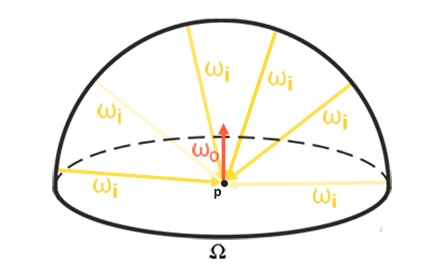
\includegraphics[scale=0.5]{hemisphere}}
        \caption{hemisphere}
      \end{figure}
      \singlespacing
    
    La ecuaci\'on de render describe la radiancia de salida sobre un punto.
    \begin{equation}
    L_o(p, w_o) = \int_{\Omega} f_r(p, w_i, w_o)L_i(p, w_i)n\cdot{w_i}dw_i
    \end{equation}
    \singlespacing
    
    Siendo $\Omega$ la hemiesfera centrada en el punto sobre la que calculamos la irradiancia,
    $f_r$ representa el BRDF, $Li$, la irradiancia de la escena, mientras que $n\cdot{w_i}$ toma en
    cuenta el \'angulo entre la de incidencia de la luz sobre la superficie.
    
    \begin{equation}
    L_o(p, w_o) = \int_{\Omega} (k_d + \frac{c}{\pi} + 
    k_s \frac{DFG}{4(w_o\cdot{n})(w_i\cdot{n})})L_i(p, w_i)n\cdot{w_i}dw_i
    \end{equation}
    \singlespacing
    
    Los terminos $k_s$ y $k_d$ de la ecuacion de reflectancia son independientes, por lo que, de la
    misma forma que en la iluminacion directa, los componentes se pueden separar en difuso y
    especular.
    
    \begin{equation}
    L_o(p, w_o) = \int_{\Omega}
    (k_d \frac{c}{\pi}) L_i(p, w_i)n\cdot{w_i}dw_i +
    \int_{\Omega} 
    k_s \frac{DFG}{4(w_o\cdot{n})(w_i\cdot{n})})L_i(p, w_i)n\cdot{w_i}dw_i
    \end{equation}
    \singlespacing
    
        \subsection{Componente difusa}
        La soluci\'on de la integral de la irradiancia de salida sobre $\Omega$ requiere samplear el entorno
        en todas las direcciones posibles. Es por ello que en tiempo real, la soluci\'on consiste en
        precomputar este c\'alculo.\\
    
        Habiendo separado la ecuaci\'on para la componente difusa y especular, podemos observar que el t\'ermino del difuso
        de Lambert es constante y lo podemos sacar de la integral.
    
        \begin{equation}
        L_o(p, w_o) = \int_{\Omega}
        (k_d \frac{c}{\pi}) L_i(p, w_i)n\cdot{w_i}dw_i=
        k_d \frac{c}{\pi} \int_{\Omega}
        (L_i(p, w_i)n\cdot{w_i}dw_i
        \end{equation}
        \singlespacing
    
            \subsubsection{T\'ecnicas IBL}
            Las t\'enicas IBL (\textit{Image Based Lighting}), permiten precalcular la irradiacia del entorno tratando el entorno
            como un gran emisoror de luz, utilizando una imagenes de referencia para aproximar la luz emitida por el entorno sobre
            el punto que estamos calculando.\\

            \textbf{Mapas de irradiancia}\\
            Los mapas de irradiancia utilizan \textit{cubemaps} para muestrear en coordenadas esf\'ericas en pasos discretos la radincia
            procedente del entorno. La irradiancia se estima como la media de la radiancia en todas las direcciones $w_i$ sobre la
            hemiesfera $\Omega$ orientada en direcci\'on a la normal de la superficie, $N$. Una vez preconvolucionado el mapa de
            entorno, el resultado, conocido como mapa de irradiancia se almacena en una textura a la que se accede en tiempo
            de ejecuci\'on para consultar los resultados precalculados de irradiancia debida al entorno.

            % % y almacenarla en una nueva textura, el mapa de irradiancia. Para ello se 
            % \todo[inline]{
            %     Convolution is applying some computation to each entry in a data set considering all other entries in the data set;
            %     the data set being the scene's radiance or environment map. Thus for every sample direction in the cubemap, we take
            %     all other sample directions over the hemisphere $\Omega$ into account.
            %     To convolute an environment map we solve the integral for each output wo sample direction by discretely sampling a
            %     large number of directions wi over the hemisphere $\Omega$ and averaging their radiance. The hemisphere we build the sample
            %     directions wi from is oriented towards the output wo sample direction we're convoluting.
            % }
            % \todo[inline]{
            %     computed sum of all indirect diffuse light of the scene hitting some surface aligned along direction wo. Such a
            %     cubemap is known as an irradiance map seeing as the convoluted cubemap effectively allows us to directly sample the
            %     scene's (pre-computed) irradiance from any direction wo.
            % }

            \begin{figure}[H]
                \vspace{0.5cm}
                \centering
                \frame{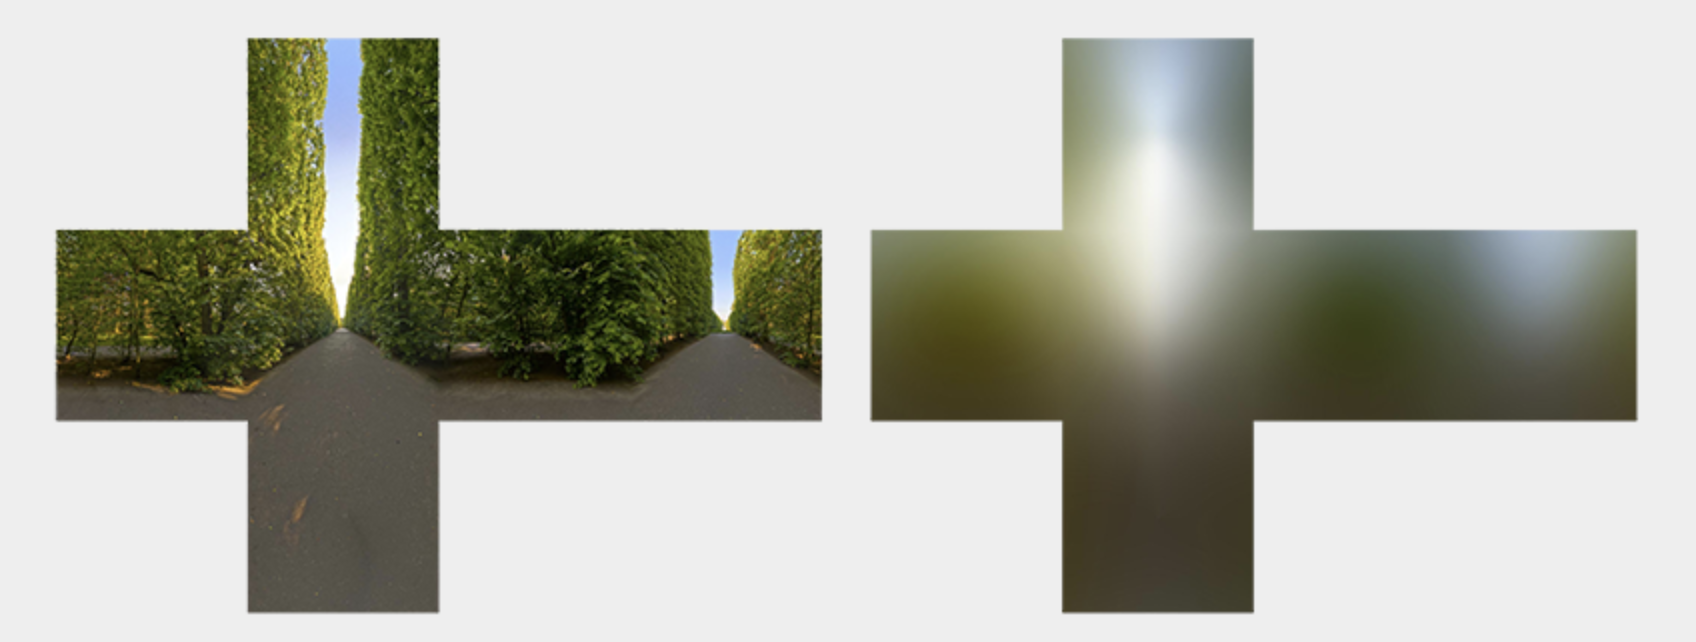
\includegraphics[scale=0.5]{irradiance_map}}
                \caption{Mapa de irradiancia como \textit{cubemap}}
            \end{figure}
            \singlespacing

            \textbf{Esf\'ericos harm\'onicos}\\
            La t\'ecnica de esf\'ericos harm\'onicos \autocite{sh} supone una optimizaci\'on sobre la t\'ecnica de mapas de irradiancia,
            que, pese a ser muy eficientes para operaciones de lectura, la convoluci\'on necesaria para generarlos tiene un coste alto.
            Los esf\'ericos harm\'onicos permiten una aproximaci\'on a la irradiancia debida al entorno comprimiendo la informaci\'on
            en una representaci\'on de espacio frente a frecuencias. De esta forma, la informaci\'on se almacena en la funci\'on de
            esf\'ericos harm\'onicos y para consultarla, se utiliza su transformada inversa, que devuelve los datos a su repesentaci\'on espacial.

            % \todo[inline]{
            %     \url{https://developer.nvidia.com/gpugems/gpugems2/part-ii-shading-lighting-and-shadows/chapter-10-real-time-computation-dynamic}
            % }

        \subsection{Componente especular}
        El m\'etodo split-sum approximation presentado por Epic \autocite{karis}, permite separar la integral en dos partes, la integral de
        la radiancia de la escena y la del BRDF. De forma similar a la componente difusa, precomputar los resultados y consultarlos y para
        calcular el resultado de la integral durante en tiempo real.\\
        
        \singlespacing
        \begin{equation}
            L_o(p, w_o) =
            \int_{\Omega}L_i(p, w_i)dw_i * \int_{\Omega}fr(p, w_i, w_o) n\cdot{w_i}dw_i
        \end{equation}
        \singlespacing

        De forma similar al mapa de irradiancia, el mapa de entorno prefiltrado se precomputa con una convoluci\'on sobre el mapa
        de entorno. La convoluci\'on utiliza la distribuci\'on de normales de Cook-Torrance \autocite{cooktorrance} en funci\'on
        de la direcci\'on de la vista, la normal y la rugosidad del material.\\
        Dado que se desconoce la direcci\'on de la vista al precomputar la radiancia, la aproximaci\'on de asume $w_i = w_o$, lo que implica perder las
        reflexiones especulares en el \'angulo cr\'itico, pero generalmente se considera una aproximaci\'on lo suficientemente buena para entornos
        interactivos. Los resultados para diferentes niveles de rugosidad se almacenan en diferentes \textit{mipmaps} de la textura.\\

        
        \begin{figure}[H]
            \vspace{0.5cm}
            \centering
            \frame{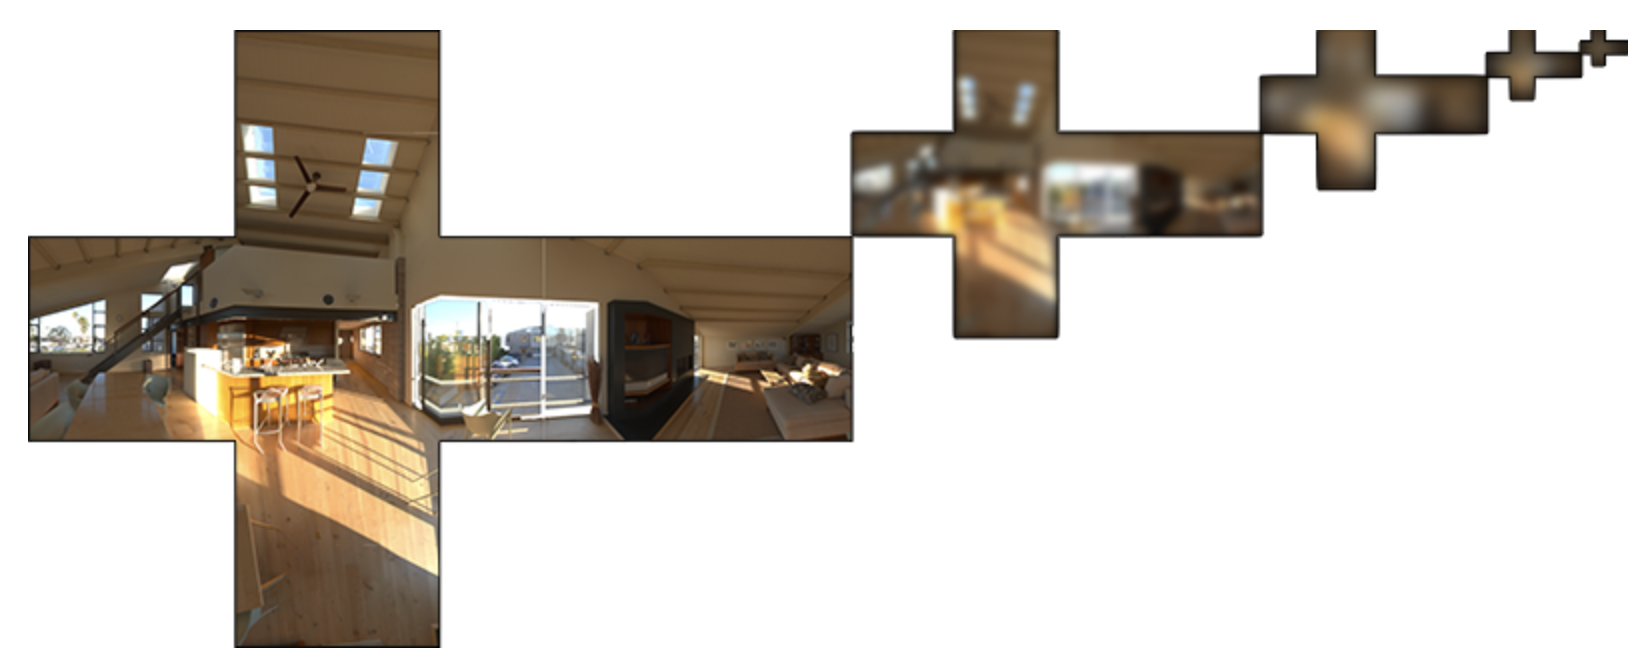
\includegraphics[scale=0.5]{prefilteredenvmap}}
            \caption{Niveles de mipmap del mapa de entorno prefiltrado en funci\'on de la rugosidad del material}
        \end{figure}
        \singlespacing

        % Para computar el mapa prefiltrado de entorno, de forma similar al mapa de irradiancia, se convoluciona el mapa de entorno
        % y se almacenan los resultados en diferentes niveles de mimaps, en funci\'on a la rugosidad de la textura.

        La segunda parte de la integral se precomputa asumiendo una radiancia blanca pura en todas direcciones, que permite calcular
        todos los posibles valores del BRDF en funci\'on de la normal de la superficie, el punto de vista y el valor de rugosidad del material.
        El resultado se almacena en un \textit{look-up texture} (LUT) que se conoce como \textit{BRDF integration map} y contiene
        valores de la escala del Fresnel en el canal rojo de la textura y valores de la desviaci\'on del Fresnel en el canal verde.
        Este LUT se consulta en tiempo de ejecuci\'on se consulta esta tabla, accediendo a sus valores utilizando rangos normalizados entre
        0 y 1 en los dos ejes, utilizando el coseno entre la vista y la normal de la superficie para el eje $x$ y valores de rugosidad
        del material en el eje $y$.

        \begin{figure}[H]
            \vspace{0.5cm}
            \centering
            \frame{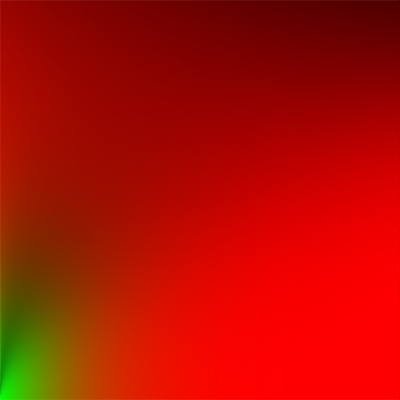
\includegraphics[scale=0.5]{brdf_lut}}
            \caption{\textit{BRDF integration map}}
        \end{figure}
        \singlespacing

        
        En tiempo de ejecuci\'on se accede a esta tabla
        utilizando los valores del coseno entre la direcci\'on de vista y la normal de la superfie en el eje $x$ y utilizando
        el valor de rugosidad del material para el eje $y$ para obtener.\\

        Finalmente el c\'alculo de la integral de la componente especular se ve reducido a una consulta al mapa de entorno prefiltrado,
        otra la \textit{BRDF integration map} y la combinacion de sus resultados:

        \singlespacing
        \begin{lstlisting}[caption=C\'alculo de la componente especular debida al entorno]
float lod = getMipLevelFromRoughness(roughness);
vec3 prefilteredColor = textureCubeLod(PrefilteredEnvMap, refVec, lod);
vec2 envBRDF = texture2D(BRDFIntegrationMap, vec2(NdotV, roughness)).xy;
vec3 indirectSpecular = prefilteredColor * (F * envBRDF.x + envBRDF.y) 
        \end{lstlisting}
        \singlespacing
        
        % un \textit{look-up texture} (LUT), que almacena
        % los c\'alculos precomputados del BRDF para los diferentes valores de \textit{rougness} y del producto escalar $w_i\cdot{n}$.
        % El \textit{BRDF integration map} asume 




        % De la misma forma que para el c\'alculo de la componente difusa, el c\'alculo de la componente especular
    


